% FONTE TEMA https://github.com/matze/mtheme
%\documentclass[aspectratio=1610]{beamer}
\documentclass[aspectratio=1610, handout]{beamer}
\usepackage[utf8]{inputenc}
\usepackage{ragged2e}
\usepackage{xcolor}
\usepackage[italian]{babel}
\usepackage{multirow}
\usepackage{silence}
\WarningFilter{beamer}{}
\WarningFilter{metropolis}{}
\usetheme[progressbar=frametitle,titleformat=smallcaps]{metropolis}
\setbeamertemplate{frame numbering}[fraction]
\setbeamercovered{dynamic}
\definecolor{rosso}{RGB}{255, 0, 0}
\definecolor{giallo}{RGB}{254,212,23}
\hypersetup{colorlinks=true,linkcolor=black,urlcolor=rosso}
\setbeamercolor{palette primary}{fg=black, bg=giallo}
\setbeamercolor{background canvas}{bg=white}
\setbeamercolor{normal text}{fg=black}
\setbeamercolor{progress bar}{fg=rosso}
\setbeamercolor{framesubtitle}{fg=rosso}
\setbeamercolor{normal text .dimmed}{fg=giallo}
\setbeamercolor{block title alerted}{fg=rosso, bg=giallo}
\setbeamerfont{caption}{size=\tiny}
\setbeamerfont{caption name}{size=\tiny}
\setlength{\abovecaptionskip}{0pt}
\makeatletter
\metroset{block=fill}
\setlength{\metropolis@progressinheadfoot@linewidth}{1pt} 
\setlength{\metropolis@progressonsectionpage@linewidth}{1pt}
\setlength{\metropolis@titleseparator@linewidth}{1pt}
\makeatother

\title{GLI ELEMENTI BASE DEGLI ALGORITMI}
\subtitle{Variabili, definizioni, assegnazioni, operazioni principali}
\date{}
\institute{\textit{
        Fonti:
        \begin{itemize}
            \item[-] \href{http://www.flowgorithm.org/documentation}{Documentazione Flowgorithm}
            \item[-] \href{https://catalogo.sanoma.it/si-op-104157-dal-bit-all-intelligenza-artificiale.html\#bundles.tab}{Dal Bit all'Intelligenza Artificiale}
        \end{itemize}
    }
}

\begin{document}

\begin{frame}[plain, noframenumbering]
    \titlepage
\end{frame}

\section{VARIABILI}

\begin{frame}{VARIABILI}
    \begin{columns}
        \column{.6\textwidth}
            \begin{alertblock}{DEFINIZIONE}
                \begin{minipage}{0.96\linewidth}
                    \justifying
                    Le \textbf{variabili} sono gli oggetti elaborati dalle istruzioni del programma. 
                    Esse risiedono nella memoria dell'elaboratore e corrispondono a \textbf{contenitori} di 
                    valori che sono utilizzati durante l'esecuzione del programma.\\
                    Alle variabili è associato un nome, detto \textbf{identificatore}, che le individua 
                    univocamente all'interno del programma. \\
                    Una variabile è quindi un contenitore di dati destinato a memorizzare valori di diverso 
                    \textbf{tipo}, il valore contenuto al suo interno può essere modificato durante l'esecuzione 
                    di un programma.
                \end{minipage}
            \end{alertblock}
        \column{.4\textwidth}
            \begin{figure}
                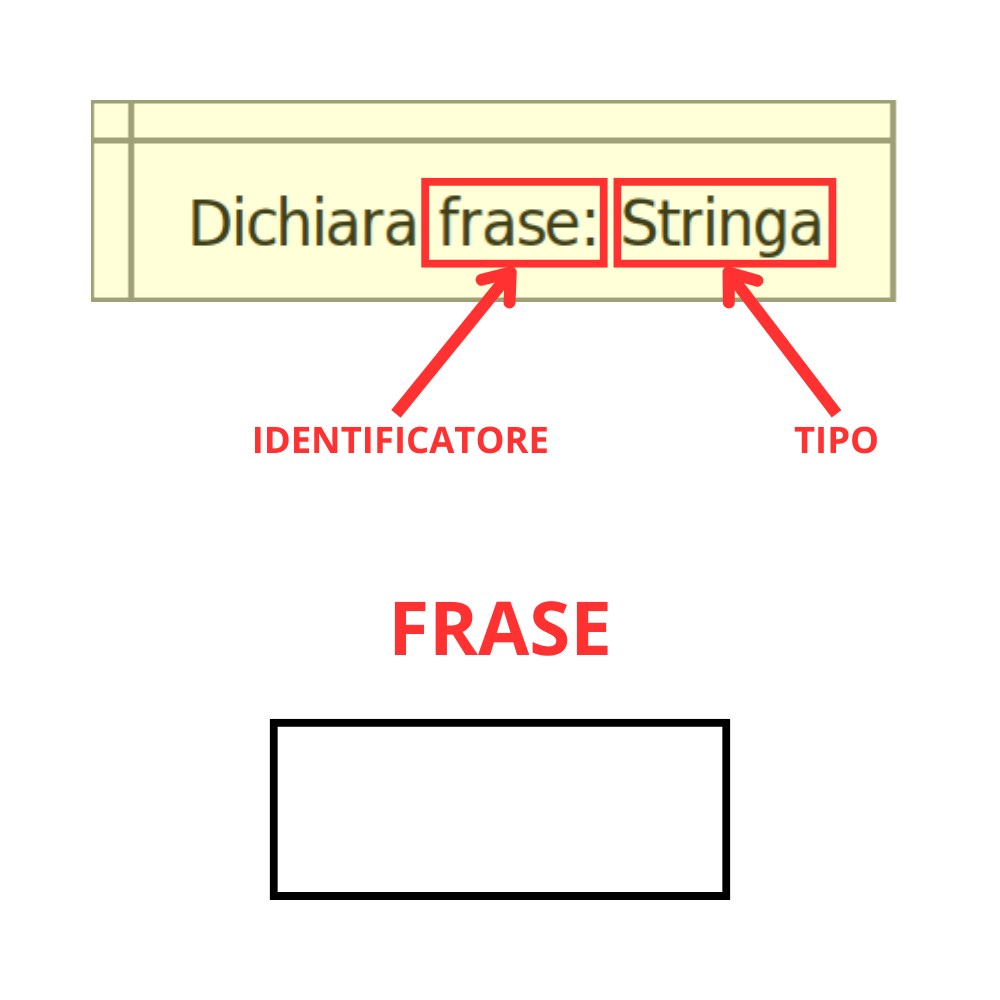
\includegraphics[width=\linewidth]{img/variabile.png}
                \caption{{creata con \href{www.canva.com}{Canva}}}
            \end{figure}
    \end{columns}
\end{frame}

\begin{frame}{TIPOLOGIE DI VARIABILI (Flowgorithm)}
    \begin{itemize}
        \item \textbf{INTERO}: un numero senza la virgola;
        \pause
        \item \textbf{REALE}: un numero con la virgola;
        \pause
        \item \textbf{STRINGA}: un insieme di caratteri (lettere, numeri, simboli) racchiusi tra doppi apici;
        \pause
        \item \textbf{BOOLEANO}: può assumere solo due valori: VERO (\textbf{TRUE}) o FALSO (\textbf{FALSE}).
    \end{itemize}
\end{frame}

\begin{frame}{DICHIARAZIONE}
    \begin{columns}
        \column{.5\textwidth}
            \begin{alertblock}{DEFINIZIONE}
                \begin{minipage}{0.96\linewidth}
                    \justifying
                    Le variabili devono essere \textbf{dichiarate} prima di essere utilizzate, 
                    specificando il loro \textbf{tipo} e il loro \textbf{identificatore} (nome).
                \end{minipage}
            \end{alertblock}
        \column{.5\textwidth}
            \begin{figure}
                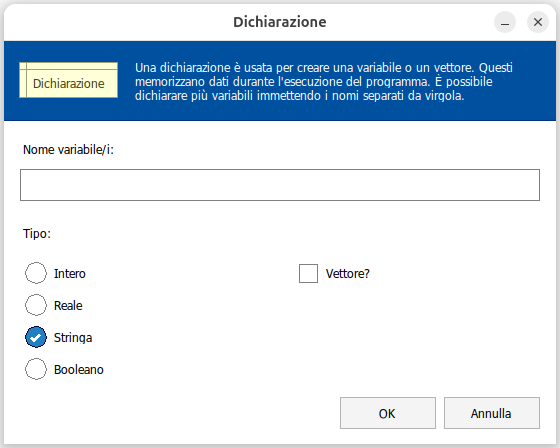
\includegraphics[width=\linewidth]{img/dichiarazione.png}
                \caption{{creata con \href{http://www.flowgorithm.org/}{Flowgorithm}}}
            \end{figure}
    \end{columns}
\end{frame}

\begin{frame}{DICHIARAZIONE}
    \begin{figure}
        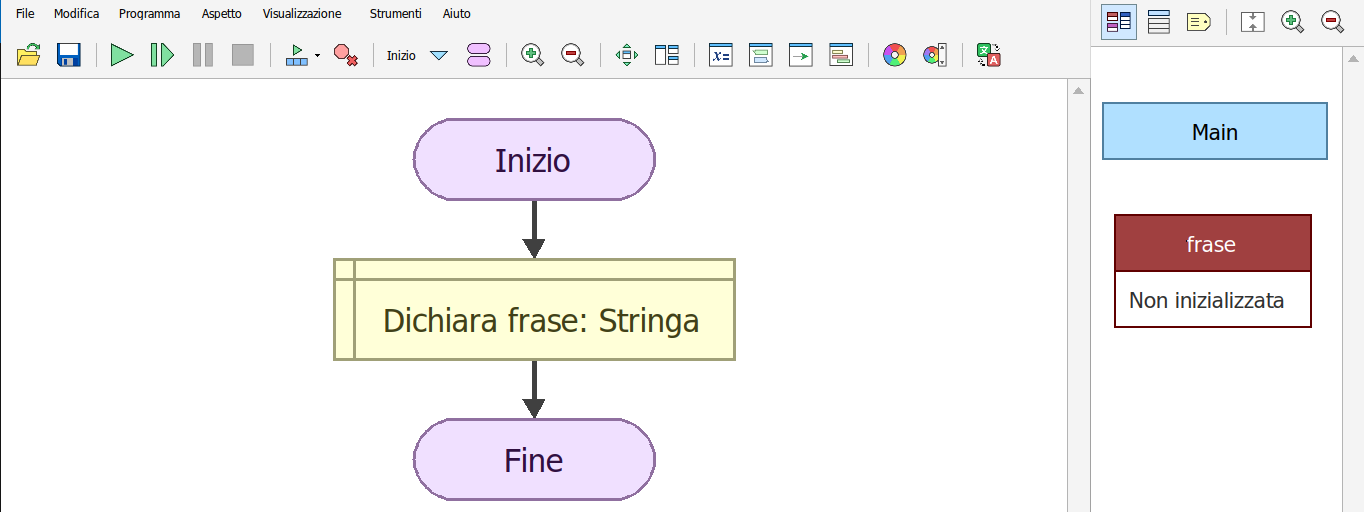
\includegraphics[width=\linewidth]{img/dichiarazione2.png}
        \caption{{creata con \href{http://www.flowgorithm.org/}{Flowgorithm}}}
    \end{figure}
\end{frame}

\begin{frame}{ASSEGNAZIONE}
    \begin{columns}
        \column{.5\textwidth}
            \begin{alertblock}{DEFINIZIONE}
                \begin{minipage}{0.96\linewidth}
                    \justifying
                    L'\textbf{assegnazione} di un valore a una variabile avviene tramite 
                    l'operatore di assegnazione \textbf{=}, che corrisponde all'inserimento 
                    di un valore nel contenitore associato all'identificatore della variabile, 
                    sostituendo il valore eventualmente già presente.\\
                    La prima assegnazione a una variabile viene detta: \textbf{inizializzazione}.
                \end{minipage}
            \end{alertblock}
        \column{.5\textwidth}
            \begin{figure}
                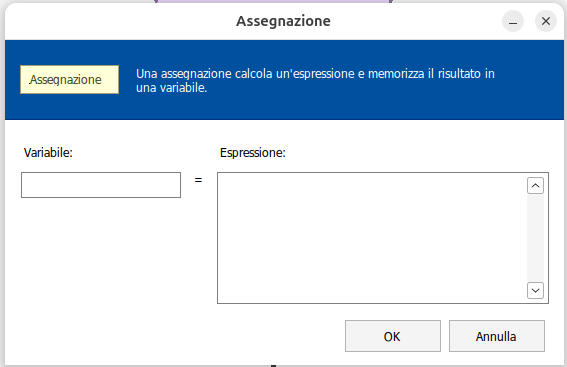
\includegraphics[width=\linewidth]{img/assegnazione.png}
                \caption{{creata con \href{http://www.flowgorithm.org/}{Flowgorithm}}}
            \end{figure}
    \end{columns}
\end{frame}

\begin{frame}{ASSEGNAZIONE}
    \begin{figure}
        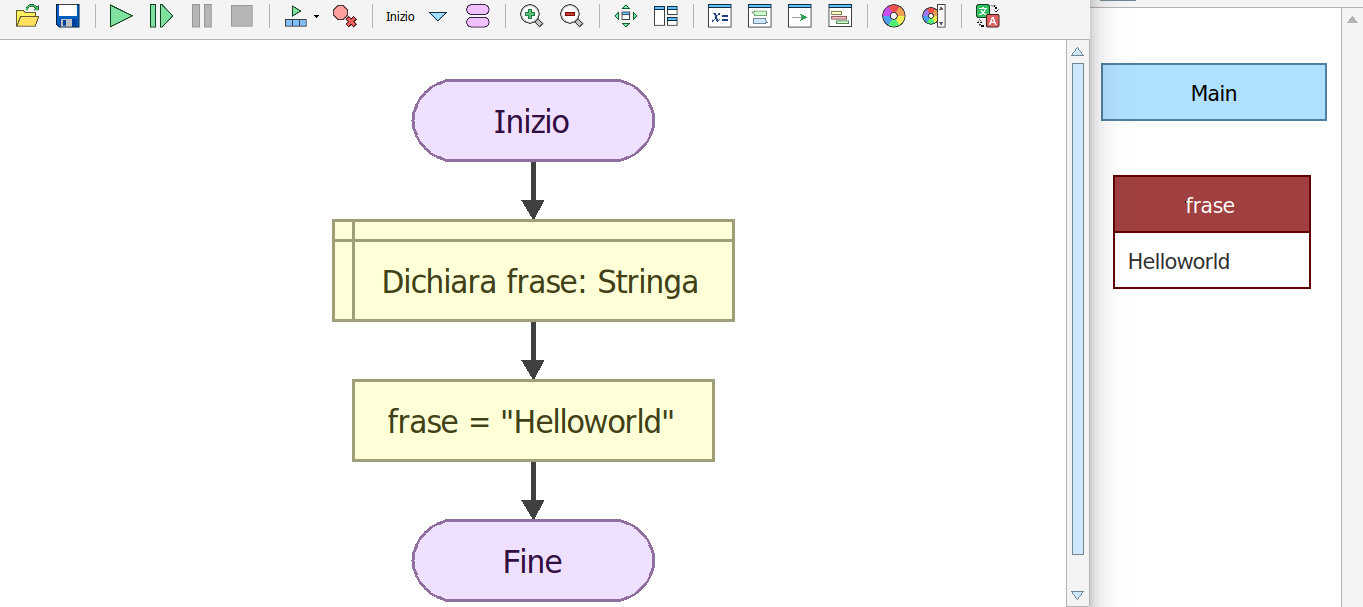
\includegraphics[width=\linewidth]{img/assegnazione2.png}
        \caption{{creata con \href{http://www.flowgorithm.org/}{Flowgorithm}}}
    \end{figure}
\end{frame}

\begin{frame}{ESEMPIO IN PSEUDOCODICE}
    \begin{figure}
        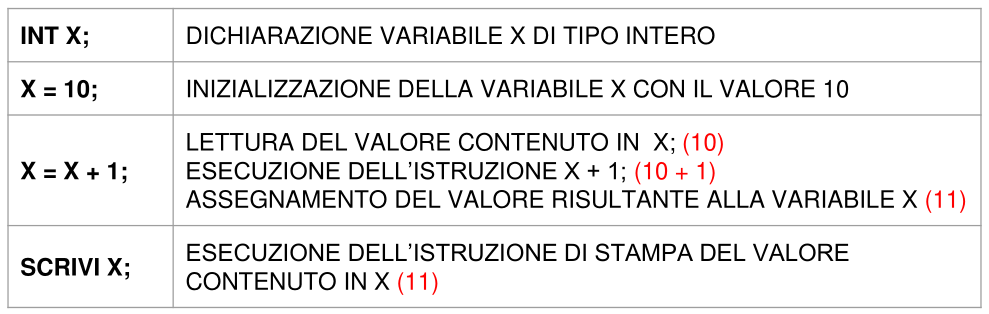
\includegraphics[width=\linewidth]{img/pseudocodice.png}
        \caption{{creata con \href{www.canva.com}{Canva}}}
    \end{figure}
\end{frame}

\section{INPUT/OUTPUT}

\begin{frame}{INPUT}
    \begin{columns}
        \column{.5\textwidth}
            \begin{alertblock}{DEFINIZIONE}
                \begin{minipage}{0.96\linewidth}
                    \justifying
                    Per \textbf{leggere} un valore in INPUT si utilizza l’istruzione di 
                    \textbf{LETTURA}, che blocca l’esecuzione del programma in attesa di un valore che 
                    deve essere inserito dall'utente. \textbf{Una volta letto il valore esso viene assegnato a una 
                    variabile definita in precedenza nel programma}.
                \end{minipage}
            \end{alertblock}
        \column{.5\textwidth}
            \begin{figure}
                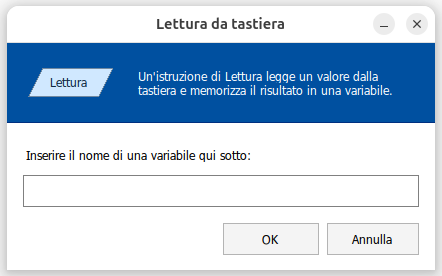
\includegraphics[width=\linewidth]{img/input.png}
                \caption{{creata con \href{http://www.flowgorithm.org/}{Flowgorithm}}}
            \end{figure}
    \end{columns}
\end{frame}

\begin{frame}{INPUT}
    \begin{figure}
        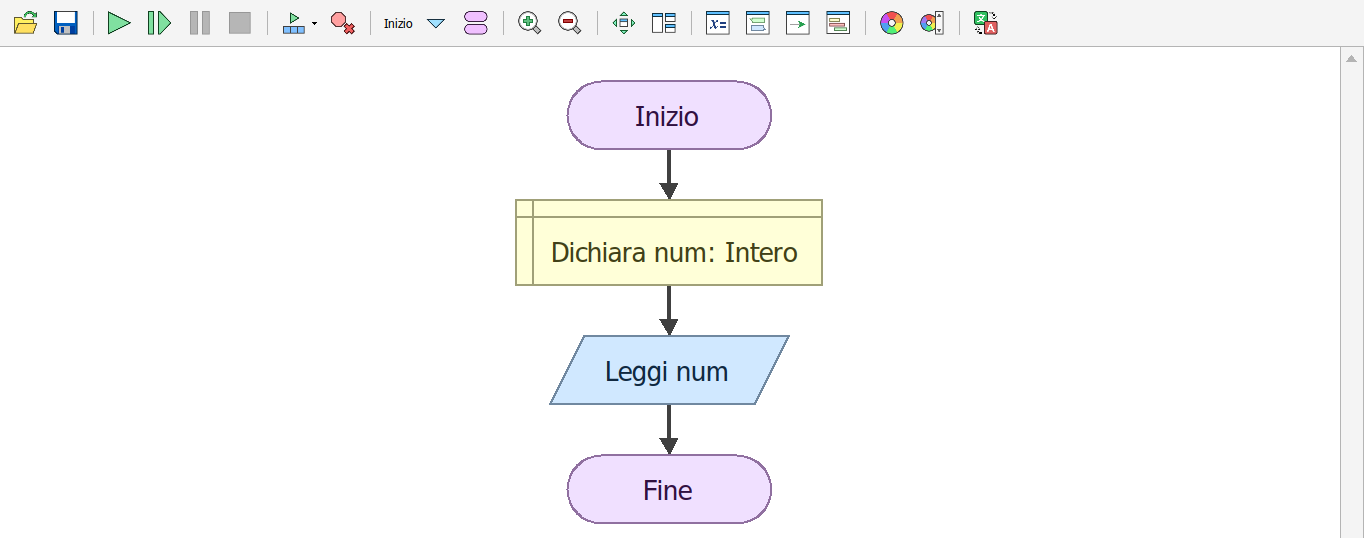
\includegraphics[width=\linewidth]{img/input2.png}
        \caption{{creata con \href{http://www.flowgorithm.org/}{Flowgorithm}}}
    \end{figure}
\end{frame}

\begin{frame}{OUTPUT}
    \begin{columns}
        \column{.5\textwidth}
            \begin{alertblock}{DEFINIZIONE}
                \begin{minipage}{0.96\linewidth}
                    \justifying 
                    Per \textbf{scrivere} un valore in OUTPUT si 
                    utilizza l’istruzione di \textbf{SCRITTURA} che stampa a 
                    video il valore desiderato.
                \end{minipage}
            \end{alertblock}
        \column{.5\textwidth}
            \begin{figure}
                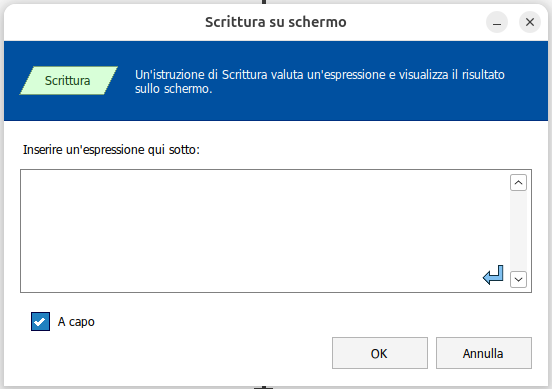
\includegraphics[width=\linewidth]{img/output.png}
                \caption{{creata con \href{http://www.flowgorithm.org/}{Flowgorithm}}}
            \end{figure}
    \end{columns}
\end{frame}

\begin{frame}{OUTPUT}
    \begin{figure}
        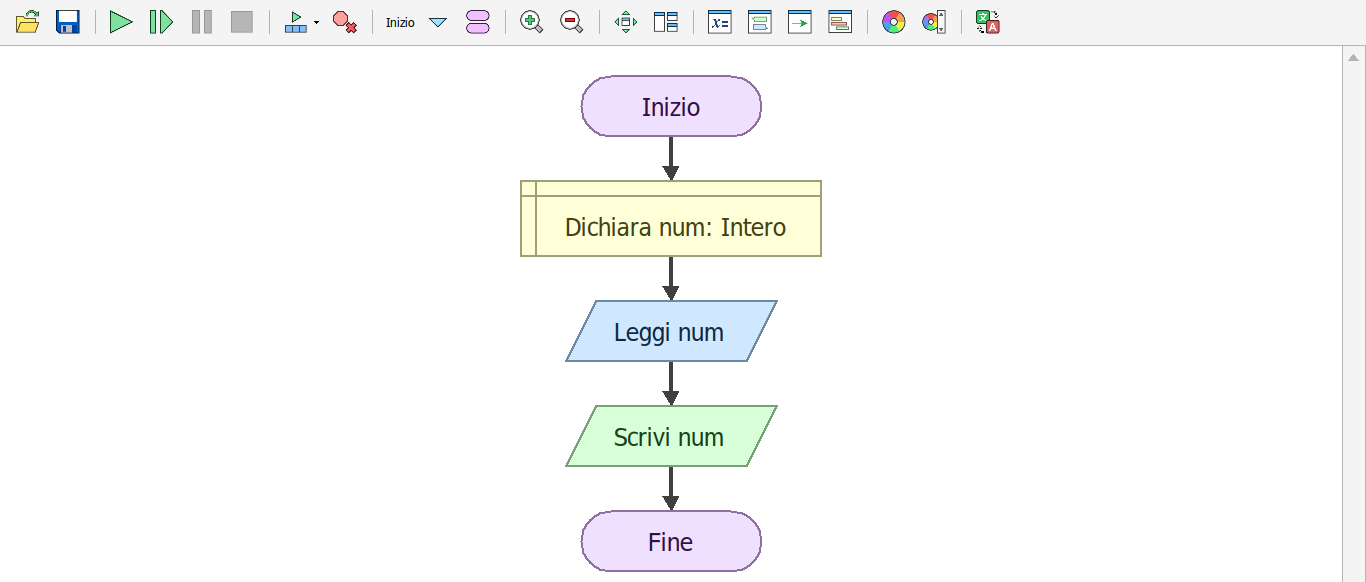
\includegraphics[width=\linewidth]{img/output2.png}
        \caption{{creata con \href{http://www.flowgorithm.org/}{Flowgorithm}}}
    \end{figure}
\end{frame}

\section{OPERAZIONI}

\begin{frame}{OPERAZIONI ARITMETICHE}
    \centering
    ESEMPIO: \textbf{A = 10} e \textbf{B = 4} \\
    \bigskip
    \begin{tabular}{c|c|c}
        \pause
        \textbf{SIMBOLO} & \textbf{OPERAZIONE} & \textbf{RISULTATO} \\
        \hline
        \hline
        \pause
        + & SOMMA & A + B risultato 14 \\
        \hline
        \pause
        - & SOTTRAZIONE & A - B risultato 6 \\
        \hline
        \pause
        * & PRODOTTO & A * B risultato 40 \\
        \hline
        \pause
        / & DIVISIONE & A / B risultato 2 \\
        \hline
        \pause
        \% & MODULO (resto) & A \% B risultato 2 \\
        \hline
    \end{tabular}
\end{frame}

\begin{frame}{OPERAZIONI DI CONFRONTO}
    \centering
    ESEMPIO: \textbf{A = 10} e \textbf{B = 4} \\
    \bigskip
    \begin{tabular}{c|c|c}
        \pause
        \textbf{SIMBOLO} & \textbf{OPERAZIONE} & \textbf{RISULTATO} \\
        \hline
        \hline
        \pause
        $>$ & MAGGIORE & A $>$ B risultato TRUE \\
        \hline
        \pause
        $<$ & MINORE & A $<$ B risultato FALSE \\
        \hline
        \pause
        = & UGUALE & A = B risultato FALSE \\
        \hline
        \pause
        != & DIVERSO & A != B risultato TRUE \\
        \hline
    \end{tabular}
\end{frame}

\begin{frame}{OPERAZIONI LOGICHE}
    \centering
    ESEMPIO: \textbf{A = 10} e \textbf{B = 4} \\
    \bigskip
    \begin{tabular}{c|c|c}
        \pause
        \textbf{SIMBOLO} & \textbf{OPERAZIONE} & \textbf{RISULTATO} \\
        \hline
        \hline
        \pause
        AND & AND LOGICO & A$<$5 AND B=4 risultato FALSE \\
        \hline
        \pause
        OR & OR LOGICO & A$<$5 OR B=4 risultato TRUE\\
        \hline
    \end{tabular}
    \bigskip
    \begin{columns}
        \column{.5\textwidth}
            \begin{tabular}{c|c|c}
                \pause
                \textbf{A} & \textbf{B} & \textbf{A AND B} \\
                \hline
                \hline
                \pause
                \textcolor{green}{TRUE} & \textcolor{green}{TRUE} & \textcolor{green}{TRUE} \\
                \hline
                \pause
                \textcolor{green}{TRUE} & \textcolor{red}{FALSE} & \textcolor{red}{FALSE} \\
                \hline
                \pause
                \textcolor{red}{FALSE} & \textcolor{green}{TRUE} & \textcolor{red}{FALSE} \\
                \hline
                \pause
                \textcolor{red}{FALSE} & \textcolor{red}{FALSE} & \textcolor{red}{FALSE} \\                
            \end{tabular}
        \column{.5\textwidth}
            \begin{tabular}{c|c|c}
                \pause
                \textbf{A} & \textbf{B} & \textbf{A OR B} \\
                \hline
                \hline
                \pause
                \textcolor{green}{TRUE} & \textcolor{green}{TRUE} & \textcolor{green}{TRUE} \\
                \hline
                \pause
                \textcolor{green}{TRUE} & \textcolor{red}{FALSE} & \textcolor{green}{TRUE} \\
                \hline
                \pause
                \textcolor{red}{FALSE} & \textcolor{green}{TRUE} & \textcolor{green}{TRUE} \\
                \hline
                \pause
                \textcolor{red}{FALSE} & \textcolor{red}{FALSE} & \textcolor{red}{FALSE} \\                
            \end{tabular}
    \end{columns}
\end{frame}

\begin{frame}{OPERAZIONE DI CONCATENAMENTO}
    \centering
    ESEMPIO: \textbf{TXT = ``RISULTATO''} e \textbf{X = 42} \\
    \bigskip
    \begin{tabular}{c|c}
        \pause
        \textbf{SIMBOLO} & \textbf{OPERAZIONE} \\
        \hline
        \hline
        \pause
        \& & CONCATENAMENTO \\
        \hline
    \end{tabular} \\
    \bigskip
    \begin{tabular}{c|c}
        \pause
        \textbf{OPERAZIONE} & \textbf{RISULTATO} \\
        \hline
        \hline
        \pause
        TXT \& X & RISULTATO42 \\
        \hline
        \pause
        TXT \& `` '' \& X & RISULTATO 42 \\
        \hline
        \pause
        ``il '' \& TXT \& `` è: '' \& X & il RISULTATO è: 42 \\
        \hline
    \end{tabular}
\end{frame}

\end{document}